\chapter{Implementazione e prove sperimentali}

\begin{figure}[H] 
    \captionsetup{justification=centering, margin=2cm, font=footnotesize}
    \begin{center}
        \makebox[0.4\paperwidth]{
            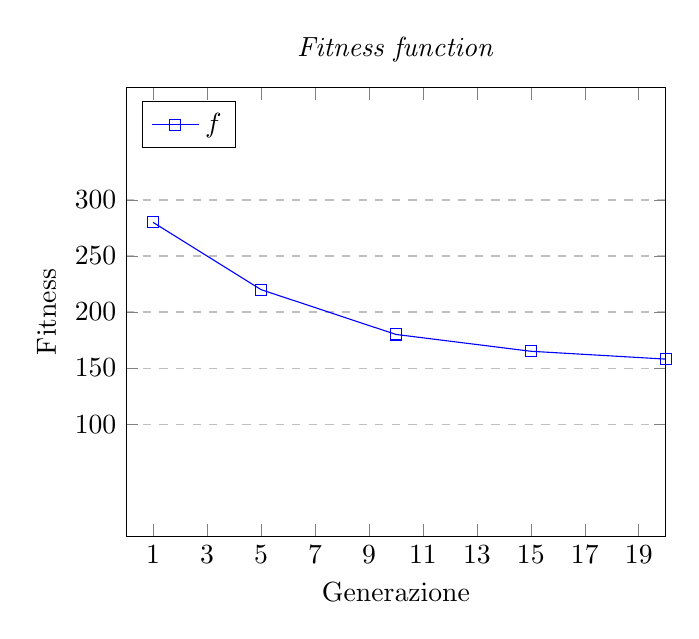
\begin{tikzpicture}
                \begin{axis}[
                    title={\textit{Fitness function}},
                    xlabel={Generazione},
                    ylabel={Fitness},
                    xmin=0, xmax=20,
                    ymin=0, ymax=400,
                    xtick={1,3,5,7,9,11,13,15,17,19},
                    ytick={100, 150, 200, 250, 300},
                    legend pos=north west,
                    ymajorgrids=true,
                    grid style=dashed,
                ]
                
                \addplot[
                    color=blue,
                    mark=square,
                    ]
                    coordinates {
                    (1,280)(5,220)(10,180)(15,165)(20,158)
                    };
                    \legend{$f$}
                
                \end{axis}
            \end{tikzpicture}
        }
    \end{center}
    \caption{Andamento della funzione obiettivo al variare di generazione.}
    \label{modello3d_feromone}
\end{figure}   
    